\section{Distributed, Collaborative, Versioned Editing}\label{sec:editing}

For the \pn project, we have developed and are hosting on \sys
\begin{compactenum}
\item the ``Math-in-the-Middle ontology''~\cite{MitM:on}, which hosts a flexiformal
  development of the mathematical knowledge for system interoperability in \pn
  (see~\cite{DehKohKon:iop16,ODK-D6.2}),
\item the ``ODK System ontologies''~\cite{ODKsysonto:on}, a collection of \omdoc/\mmt
  theories and codecs that describe the mathematical content of the LMFDB and other data
  sources, bridging the internal (i.e. system/database oriented) and external
  (mathematical) views of the content.
\end{compactenum}
These two \sys libraries are in an early state currently and curating them is a major task
in in work package \textbf{WP6} of the \pn project. Therefore the editing workflows are
crucial to the project.

Given the distributed and collaborative nature of the \pn project, the editing facilities
need to be as well. As experience in sortware engineering shows -- and flexiformal active
documents are like software in many respects -- this is only possible using (concepts of)
revision control systems. In \sys we took the major design decision to use the distributed
revision control system GIT~\cite{GIT:on} as the basis for all general storage,
authentification, distribution, and collaboration functionalities and build
domain-specific functionality on top of that. We took the minor design decision to use the
GitLab~\cite{GitLab:on} system as the repository management system -- rather than e.g.
GtiHub~\cite{GitHub:on}, since it is open source and allows us to run our own server and
configure it more by patching the code.

We organize the content into \textbf{libraries} by area or intended application --
e.g. the two libraries discussed at the top of this section and further divide them up
into \textbf{math archives}~\cite{HorIacJuc:cscpnrr11}, which standardize the file system
layout of all dimensions of mathematical representations: source, content, presentation,
narration, \ldots. At the GitLab level, libraries are modeled as ``groups'' and individual
math archives as repositories. As GIT -- and thus repository managers like GitLab -- only
allow authentification at the repository level, math archives are mostly used for
authentification and access control in \sys.

The advantage of the GIT-based setup is that we can combine two methods for accessing the
contents of \sys:
\begin{compactenum}[\em i\rm)]
\item an online, web-based editing/interaction workflow for the casual user, in the spirit
  of the Planetary system and
\item an offline editing/authoring workflow based on a GIT working copy.
\end{compactenum}
We will describe both separately in sections~\ref{sec:lmh} and \ref{sec:web}, after
clarify the setting in \sys a bit more. 

\subsection{Building a Math Knowledge Base by Editing Surface Language Documents}\label{sec:surface}

The unifying representation format of the \sys system is flexiformal \omdoc/mmt, which is
structured as a theory graph. As \omdoc/\mmt is optimized for machine processing, actual
content is authored and edited as documents in a \textbf{surface format}: a human-oriented
syntax that can be compiled into \omdoc/\mmt. \sys currently supports five surface formats 
\begin{enumerate}
\item HTML5 and TeX/LaTeX (as a minimally flexiformal document formats)
\item \sTeX (semantic {\TeX/\LaTeX}), an extension of {\LaTeX} that allows to annotate
  {\LaTeX} documents with semantic properties and relations.
\item \mmt surface syntax.
\item TWELF (Edinburgh Logical Framework in TWELF syntax)
\end{enumerate}
Additionally, the native formats of the theorem prover libraries imported into MathHub are
handled by special importers on a system-by-system basis. Only \sTeX and \mmt syntax are
relevant for the \pn project, so we will ignore the others in this report. In all cases,
the conversion to \omdoc/\mmt is a multi-step, multi-document, dependency-driven process,
which is handled by the \mmt build system~\cite{mmt:buildsys:on} (see the upper right hand
corner in Figure~\ref{fig:arch}).

\subsection{Local \sys Editing}\label{sec:lmh}

The local editing workflow is important for power authors who want to edit more than one
file simultaneously or have customized modes for the surface languages in their own
editors. A user can fork or pull the relevant repositories from the \sys GitLab, edit them
and submit them back to \sys either via a pull request to the repository masters or a
direct commit/push. As the content is usually highly networked and distributed across
multiple math archives (and thus GIT repositories), we have developed a command line tool
\lmh (\underline{l}ocal \underline{M}ath\underline{H}ub; see~\cite{lmh:on}
and~\cite{lmh-docker:on} for a docker container that bundles up all system requirements
for \lmh) that manages working copies across repository borders taking into account e.g.
cross-archive dependencies. 

\lmh also supports running the build system locally and previewing HTML5 renderings of the
generated \omdoc/\mmt.

Figure~\ref{fig:jedit2} shows a JEdit-based IDE for \omdoc/\mmt content in \mmt surface
syntax that is tightly coupled with the \mmt API for semantic services;
see~\cite{Rabe:LII14} for details.

\begin{figure}[ht]\centering
  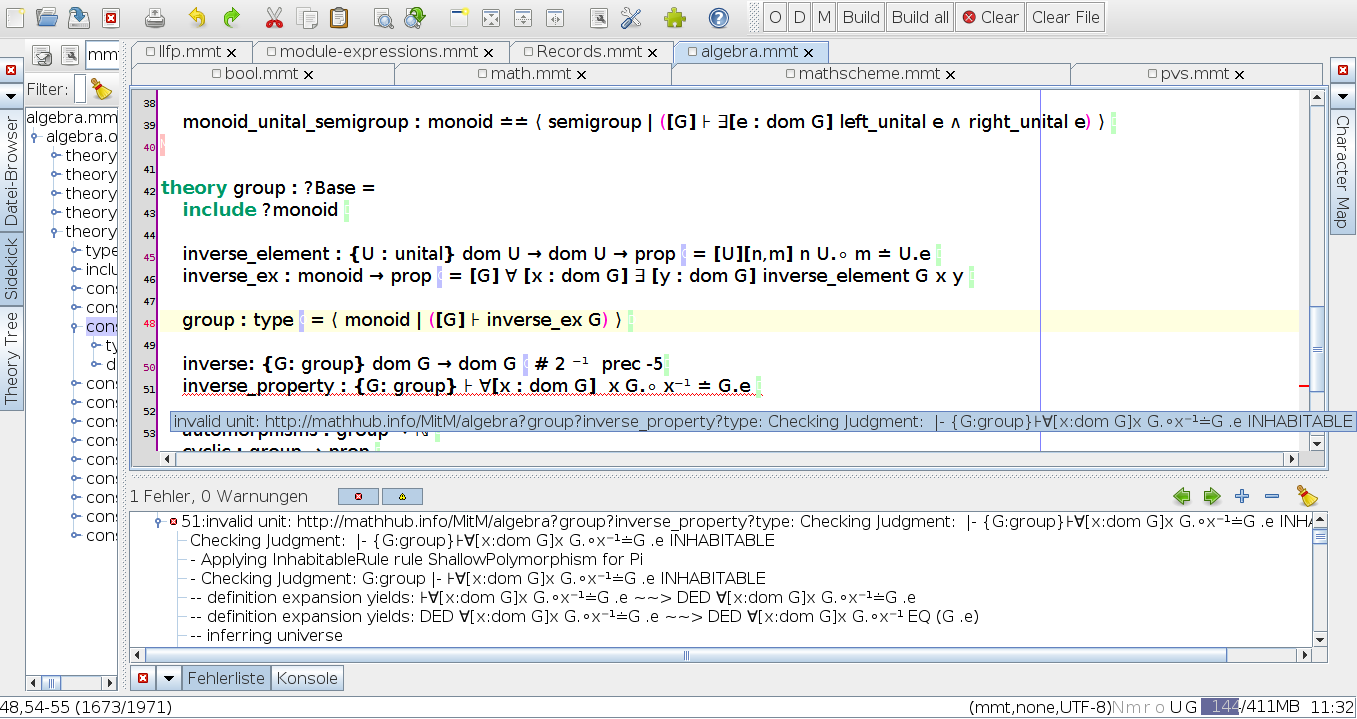
\includegraphics[width=15cm]{jedit2}
  \caption{Local Editing of \mmt Surface Syntax in JEdit}\label{fig:jedit2}
\end{figure}

\subsection{Web-based \sys Editing}\label{sec:web}

\ednote{MK: write}
%%% Local Variables:
%%% mode: latex
%%% TeX-master: "report"
%%% End:
